\chapter{Сандар теориясы}

\index{сандар теориясы}

\key{Сандар теориясы} -- математика ғылымының бүтін
сандарды зерттейтін тармағы. 
Сандар теориясы қызықты да күрделі сала. Себебі бүтін сандарға байланысты көптеген есептер бар және олар
бір қарағанда қарапайым болып көрінгенімен, шешу барысында 
өте қиын екені байқалады.
% is a branch of mathematics
% that studies integers.
% Number theory is a fascinating field,
% because many questions involving integers
% are very difficult to solve even if they
% seem simple at first glance.

Үлгі ретінде келесі теңдеуді қарастырайық:
% As an example, consider the following equation:
\[x^3 + y^3 + z^3 = 33\]
Теңдеуді қанағаттандыратын $x$, $y$ және $z$ 
үш нақты санын табу оңай.
Мысалы, біз келесі мәндерді таңдай аламыз:
% It is easy to find three real numbers $x$, $y$ and $z$
% that satisfy the equation.
% For example, we can choose
\[
\begin{array}{lcl}
x = 3, \\
y = \sqrt[3]{3}, \\
z = \sqrt[3]{3}.\\
\end{array}
\]
Дегенмен: ''теңдікті қанағаттандыратын $x$, $y$ және $z$ сандары
бар ма'' \cite{bec07} - деген сұрақ сандар теориясындағы ашық мәселе болып отыр. 
% However, it is an open problem in number theory
% if there are any three
% \emph{integers} $x$, $y$ and $z$
% that would satisfy the equation \cite{bec07}.

Тарауда сандар теориясындағы негізгі 
ұғымдар мен алгоритмдерге тоқталамыз.
Егер басқаша көрсетілмесе,
біз үшін тарау бойы барлық сандар бүтін сандар болады.

% In this chapter, we will focus on basic concepts
% and algorithms in number theory.
% Throughout the chapter, we will assume that all numbers
% are integers, if not otherwise stated.

\section{Жай сандар және көбейткіштер}

\index{бөлінгіш}
\index{көбейткіш}
\index{бөлгіш}

Егер $a$ саны $b$ санын қалдықсыз бөлсе, 
$a$ санын $b$ санының \key{көбейткіші} немесе \key{бөлгіші}
дейміз.
% of a number $b$
% if $a$ divides $b$.
Егер $a$ саны $b$ санының көбейткіші болса, 
$a \mid b$ түрінде, ал керісінше болса, $a \nmid b$ 
түрінде жазамыз.
Мысалы, 24 санының көбейткіштері: 
1, 2, 3, 4, 6, 8, 12 және 24.
% If $a$ is a factor of $b$,
% we write $a \mid b$, and otherwise we write $a \nmid b$.
% For example, the factors of 24 are
% 1, 2, 3, 4, 6, 8, 12 and 24.

\index{жай сан}
\index{жай көбейткіштерге жіктеу}

Егер $n>1$ санының жалғыз көбейткіштері 
1 және $n$ болса, ол -- \key{жай сан}.
Мысалы, 7, 19 және 41 -- жай сандар. Бірақ
35 жай сан емес, себебі $5 \cdot 7 = 35$.
Әр $n>1$ санын \key{жай көбейткіштерге бірегей жіктеуге} болады:
% if its only positive factors are 1 and $n$.

% For example, 7, 19 and 41 are primes,
% but 35 is not a prime, because $5 \cdot 7 = 35$.
% For every number $n>1$, there is a unique
% \key{prime factorization}
\[ n = p_1^{\alpha_1} p_2^{\alpha_2} \cdots p_k^{\alpha_k},\]
бұл жерде $p_1,p_2,\ldots,p_k$ -- бірегей жай сандар, ал 
$\alpha_1,\alpha_2,\ldots,\alpha_k$ -- оң сандар.
Мысалы, 84 санын жай сандарға келесі жолмен жіктейміз:
\[84 = 2^2 \cdot 3^1 \cdot 7^1.\]
% where $p_1,p_2,\ldots,p_k$ are distinct primes and
% $\alpha_1,\alpha_2,\ldots,\alpha_k$ are positive numbers.
% For example, the prime factorization for 84 is
% \[84 = 2^2 \cdot 3^1 \cdot 7^1.\]

$n$ санының \key{көбейткіштер саны}:
\[\tau(n)=\prod_{i=1}^k (\alpha_i+1),\]
себебі әр $p_i$ жай саны көбейткіште $\alpha_i+1$ ретке дейін
кездесе алады.
Мысалы, 84 санының көбейткіштер санын осылай есептейміз:
$\tau(84)=3 \cdot 2 \cdot 2 = 12$.
Оның көбейткіштері: 1, 2, 3, 4, 6, 7, 12, 14, 
21, 28, 42 және 84.
% because for each prime $p_i$, there are
% $\alpha_i+1$ ways to choose how many times
% it appears in the factor.
% For example, the number of factors
% of 84 is
% $\tau(84)=3 \cdot 2 \cdot 2 = 12$.
% The factors are
% 1, 2, 3, 4, 6, 7, 12, 14, 21, 28, 42 and 84.

$n$ санының көбейткіштер қосындысы осы формулаға тең:
\[\sigma(n)=\prod_{i=1}^k (1+p_i+\ldots+p_i^{\alpha_i}) = \prod_{i=1}^k \frac{p_i^{a_i+1}-1}{p_i-1},\]
бұл жердегі екінші формула геометриялық прогрессия формуласына
негізделген.
Мысалы, 84 санының көбейткіштерінің қосындысы:
\[\sigma(84)=\frac{2^3-1}{2-1} \cdot \frac{3^2-1}{3-1} \cdot \frac{7^2-1}{7-1} = 7 \cdot 4 \cdot 8 = 224.\]
% The \key{sum of factors} of $n$ is
% \[\sigma(n)=\prod_{i=1}^k (1+p_i+\ldots+p_i^{\alpha_i}) = \prod_{i=1}^k \frac{p_i^{a_i+1}-1}{p_i-1},\]
% where the latter formula is based on the geometric progression formula.
% For example, the sum of factors of 84 is
% \[\sigma(84)=\frac{2^3-1}{2-1} \cdot \frac{3^2-1}{3-1} \cdot \frac{7^2-1}{7-1} = 7 \cdot 4 \cdot 8 = 224.\]

$n$ санының көбейткіштер көбейтіндісінің формуласы --
\[\mu(n)=n^{\tau(n)/2}.\]
Себебі көбейтіндісі $n$ болатын 
$\tau(n)/2$ 
көбейткіштер жұптарын құра аламыз.
Мысалы, 84 санының көбейткіштері
$1 \cdot 84$, $2 \cdot 42$, $3 \cdot 28$ және т. б.
жұптарын құрайды, осылайша көбейткіштердің
көбейтіндісі $\mu(84)=84^6=351298031616$ тең.
% The \key{product of factors} of $n$ is
% \[\mu(n)=n^{\tau(n)/2},\]
% because we can form $\tau(n)/2$ pairs from the factors,
% each with product $n$.
% For example, the factors of 84
% produce the pairs
% $1 \cdot 84$, $2 \cdot 42$, $3 \cdot 28$, etc.,
% and the product of the factors is $\mu(84)=84^6=351298031616$.

\index{кемел сан}

Егер $n=\sigma(n)-n$ тең болса,
яғни $1$-ден $n-1$-ге дейінгі көбейткіштердің қосындысы
$n$ санына тең болса, $n$ санын кемел сан дейміз.
Мысалы, 28 кемел сан, себебі $28=1+2+4+7+14$.
% A number $n$ is called a \key{perfect number} if $n=\sigma(n)-n$,
% i.e., $n$ equals the sum of its factors
% between $1$ and $n-1$.
% For example, 28 is a perfect number,
% because $28=1+2+4+7+14$.

\subsubsection{Жай сандар мөлшері}

Жай сандар мөлшері шексіз екенін көрсету оңай.
Егер жай сандар шекті болса, $P=\{p_1,p_2,\ldots,p_n\}$
барлық жай сандарды қамтитын жиын құрайтын едік.
Мысалы, $p_1=2$, $p_2=3$, $p_3=5$ және дәл солай жалғаса
береді. Дегенмен $P$ жиынын қолданып біз жаңадан
\[p_1 p_2 \cdots p_n+1\] жай санын құрай аламыз.
Ал ол сан $P$ жиындағы барлық сандардан үлкен,
бұл -- қарама-қайшылық, сондықтан жай сандар мөлшері
шексіз болмақ.
% It is easy to show that there is an infinite number
% of primes.
% If the number of primes would be finite,
% we could construct a set $P=\{p_1,p_2,\ldots,p_n\}$
% that would contain all the primes.
% For example, $p_1=2$, $p_2=3$, $p_3=5$, and so on.
% However, using $P$, we could form a new prime
% \[p_1 p_2 \cdots p_n+1\]
% that is larger than all elements in $P$.
% This is a contradiction, and the number of primes
% has to be infinite.

\subsubsection{Жай сандар тығыздығы}
% \subsubsection{Desnity of primes}

Жай сандар тығыздығы -- сандар арасындағы жай сандардың
жиілігін көрсетеді.
$\pi(n)$ деп $1$-ден $n$-ге дейінгі жай сандардың санын көрсетеді.
Мысалы, $\pi(10)=4$, себебі $1$ мен $10$ арасында 4 жай сан бар. Олар:
2, 3, 5 және 7.
% The density of primes means how often there are primes
% among the numbers.
% Let $\pi(n)$ denote the number of primes between
% $1$ and $n$. For example, $\pi(10)=4$, because
% there are 4 primes between $1$ and $10$: 2, 3, 5 and 7.

Келесіні көрсетуге болды:

\[\pi(n) \approx \frac{n}{\ln n}.\]
Бұл жай сандардың жиі кездесетінін байқатады.
Мысалы, $1$ және $10^6$ арасындағы 
жай сандар мөлшері $\pi(10^6)=78498$ тең және 
$10^6 / \ln 10^6 \approx 72382$.
% It is possible to show that
% \[\pi(n) \approx \frac{n}{\ln n},\]
% which means that primes are quite frequent.
% For example, the number of primes between
% $1$ and $10^6$ is $\pi(10^6)=78498$,
% and $10^6 / \ln 10^6 \approx 72382$.

\subsubsection{Гипотеза}

Жай сандарға қатысты көптеген гипотезалар бар.
Көп адамдар гипотезаларды шындық деп санайды, 
бірақ оны ешкім әлі дәлелдей алмады. Мысалы, бізге белгілі келесі
гипотезалар бар:
% There are many \emph{conjectures} involving primes.
% Most people think that the conjectures are true,
% but nobody has been able to prove them.
% For example, the following conjectures are famous:

\begin{itemize}
\index{Голдбах гипотезасы}
\item \key{Голдбах гипотезасы}:
әр $n>2$ жұп бүтін саны
$a$ және $b$ жай сандардың қосындысына тең.
\index{егіз сандар}
\item \key{Егіз сандар гипотезасы}:
$p$ және $p+2$ жай сан болатындай
$\{p,p+2\}$ түріндегі жұптардың шексіз саны бар.
\index{Лежандр гипотезасы}
\item \key{Лежандр гипотезасы}:
$n$ саны оң бүтін сан болса,
$n^2$ және $(n+1)^2$ арасында әрқашанда жай сан болады.
\end{itemize}

% \begin{itemize}
% \index{Goldbach's conjecture}
% \item \key{Goldbach's conjecture}:
% Each even integer $n>2$ can be represented as a
% sum $n=a+b$ so that both $a$ and $b$ are primes.
% \index{twin prime}
% \item \key{Twin prime conjecture}:
% There is an infinite number of pairs
% of the form $\{p,p+2\}$,
% where both $p$ and $p+2$ are primes.
% \index{Legendre's conjecture}
% \item \key{Legendre's conjecture}:
% There is always a prime between numbers
% $n^2$ and $(n+1)^2$, where $n$ is any positive integer.
% \end{itemize}

\subsubsection{Негізгі алгоритмдер}

Егер $n$ саны жай сан болмаса, 
оны $a \cdot b$ көбейтіндісі ретінде 
көрсетуге болады.
Бұл жерде $a \le \sqrt n$ немесе $b \le \sqrt n$, 
демек бұл сан $2$ мен $\lfloor \sqrt n \rfloor$ арасында
көбейткішті қамтиды.
Осы бақылау арқылы біз санды жай санға $O(\sqrt n)$ уақытта
тексере аламыз. Одан басқа, санды жай сандарға да $O(\sqrt n)$
уақытта жіктей аламыз.
% If a number $n$ is not prime,
% it can be represented as a product $a \cdot b$,
% where $a \le \sqrt n$ or $b \le \sqrt n$,
% so it certainly has a factor between $2$ and $\lfloor \sqrt n \rfloor$.
% Using this observation, we can both test
% if a number is prime and find the prime factorization
% of a number in $O(\sqrt n)$ time.

Келесі \texttt{prime} функциясы $n$ саны жай сан екендігіне
тексереді. Функция $n$ санын $2$ мен $\lfloor \sqrt n \rfloor$
арасындағы барлық сандарға бөліп көреді. Соның арасындағы
еш сан бөлмесе, онда $n$ саны жай сан болады.
% The following function \texttt{prime} checks
% if the given number $n$ is prime.
% The function attempts to divide $n$ by
% all numbers between $2$ and $\lfloor \sqrt n \rfloor$,
% and if none of them divides $n$, then $n$ is prime.

\begin{lstlisting}
bool prime(int n) {
    if (n < 2) return false;
    for (int x = 2; x*x <= n; x++) {
        if (n%x == 0) return false;
    }
    return true;
}
\end{lstlisting}

\noindent
Келесі \texttt{factors} функциясы 
$n$ санын жай сандарға жіктеген кездегі
жай сандарды қамтитын векторды құрайды.
Функция $n$ санды оның жай сан болатын
көбейткіштеріне бөледі және соларды векторға қосады.
Егер қалған $n$ саны
$2$ мен $\lfloor \sqrt n \rfloor$ арасындағы 
көбейткіштерді қамтымаса, бұл процесс аяқталады. Егер $n>1$, 
ол жай сан және соңғы көбейткіш болады.
% The following function \texttt{factors}
% constructs a vector that contains the prime
% factorization of $n$.
% The function divides $n$ by its prime factors,
% and adds them to the vector.
% The process ends when the remaining number $n$
% has no factors between $2$ and $\lfloor \sqrt n \rfloor$.
% If $n>1$, it is prime and the last factor.

\begin{lstlisting}
vector<int> factors(int n) {
    vector<int> f;
    for (int x = 2; x*x <= n; x++) {
        while (n%x == 0) {
            f.push_back(x);
            n /= x;
        }
    }
    if (n > 1) f.push_back(n);
    return f;
}
\end{lstlisting}

Әрбір жай көбейткіштің векторда санды қанша бөлсе, 
сонша рет пайда болатынын ескергеніміз жөн.
Мысалға, $24=2^3 \cdot 3$ сондықтан функцияның вектордағы
элементтері $[2,2,2,3]$ болады.
% Note that each prime factor appears in the vector
% as many times as it divides the number.
% For example, $24=2^3 \cdot 3$,
% so the result of the function is $[2,2,2,3]$.

\subsubsection{Эратосфен елегі}

\index{Эратосфен елегі}

\key{Эратосфен елегі}
%\footnote{Eratosthenes (c. 276 BC -- c. 194 BC) was a Greek mathematician.}
дегеніміз $2 \ldots n$ арасындағы сан жай сан екендігін тиімді тексеруге
көмектесетін жиымды құрайтын алдын ала өңдеу алгоритмі.
% is a preprocessing
% algorithm that builds an array using which we
% can efficiently check if a given number between $2 \ldots n$
% is prime and, if it is not, find one prime factor of the number.

Алгоритм $2,3,\ldots,n$ позициялары қолданылатын жиым елегін құрайды.

% The algorithm builds an array $\texttt{sieve}$
% whose positions $2,3,\ldots,n$ are used.
$\texttt{sieve}[k]=0$ деген мән $k$ саны жай сан екенін
білдіреді, ал керісінше, $\texttt{sieve}[k] \neq 0$ мәні сан жай сан емес
екенін білдіріп, осы санның бір жай көбейтіші $\texttt{sieve}[k]$ екенін
тауып береді.
% The value $\texttt{sieve}[k]=0$ means
% that $k$ is prime,
% and the value $\texttt{sieve}[k] \neq 0$
% means that $k$ is not a prime and one
% of its prime factors is $\texttt{sieve}[k]$.

Алгоритм $2 \ldots n$ арасындағы сандарды
біртіндеп жүріп шығады.
$x$ жай саны табылған кезде, алгоритм $x$ санының
еселіктерін жай сан емес деп белгілейді. Себебі, оларды
$x$ саны бөледі.
% The algorithm iterates through the numbers
% $2 \ldots n$ one by one.
% Always when a new prime $x$ is found,
% the algorithm records that the multiples
% of $x$ ($2x,3x,4x,\ldots$) are not primes,
% because the number $x$ divides them.

Мысалға, егер $n=20$, жиым осындай болады:
% For example, if $n=20$, the array is as follows:

\begin{center}
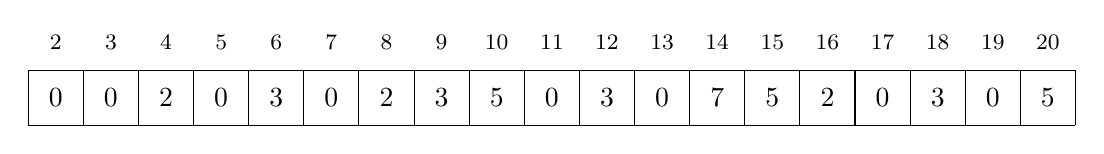
\begin{tikzpicture}[scale=0.7]
\draw (0,0) grid (19,1);

\node at (0.5,0.5) {$0$};
\node at (1.5,0.5) {$0$};
\node at (2.5,0.5) {$2$};
\node at (3.5,0.5) {$0$};
\node at (4.5,0.5) {$3$};
\node at (5.5,0.5) {$0$};
\node at (6.5,0.5) {$2$};
\node at (7.5,0.5) {$3$};
\node at (8.5,0.5) {$5$};
\node at (9.5,0.5) {$0$};
\node at (10.5,0.5) {$3$};
\node at (11.5,0.5) {$0$};
\node at (12.5,0.5) {$7$};
\node at (13.5,0.5) {$5$};
\node at (14.5,0.5) {$2$};
\node at (15.5,0.5) {$0$};
\node at (16.5,0.5) {$3$};
\node at (17.5,0.5) {$0$};
\node at (18.5,0.5) {$5$};

\footnotesize

\node at (0.5,1.5) {$2$};
\node at (1.5,1.5) {$3$};
\node at (2.5,1.5) {$4$};
\node at (3.5,1.5) {$5$};
\node at (4.5,1.5) {$6$};
\node at (5.5,1.5) {$7$};
\node at (6.5,1.5) {$8$};
\node at (7.5,1.5) {$9$};
\node at (8.5,1.5) {$10$};
\node at (9.5,1.5) {$11$};
\node at (10.5,1.5) {$12$};
\node at (11.5,1.5) {$13$};
\node at (12.5,1.5) {$14$};
\node at (13.5,1.5) {$15$};
\node at (14.5,1.5) {$16$};
\node at (15.5,1.5) {$17$};
\node at (16.5,1.5) {$18$};
\node at (17.5,1.5) {$19$};
\node at (18.5,1.5) {$20$};

\end{tikzpicture}
\end{center}

Эратосфен елегiнің коды келесі ретпен жазылады.
Код \texttt{sieve} жиымының әрбір элементін 
бастапқыда нөлге тең деп есептейді.
% The following code implements the sieve of
% Eratosthenes.
% The code assumes that each element of
% \texttt{sieve} is initially zero.

\begin{lstlisting}
for (int x = 2; x <= n; x++) {
    if (sieve[x]) continue;
    for (int u = 2*x; u <= n; u += x) {
        sieve[u] = x;
    }
}
\end{lstlisting}

Алгоритмнің ішкі қайталымы әр $x$ мәніне $n/x$ рет орындалады.
Сондықтан алгоритмнің орындалу уақытының жоғарғы шегі гармоникалық
қосынды деп саналады:
% The inner loop of the algorithm is executed
% $n/x$ times for each value of $x$.
% Thus, an upper bound for the running time
% of the algorithm is the harmonic sum
\[\sum_{x=2}^n n/x = n/2 + n/3 + n/4 + \cdots + n/n = O(n \log n).\]

\index{гармоникалық
қосынды}

Ішкі қайталым тек 
$x$ саны жай болғанда ғана орындалатындықтан, бұл алгоритм шынымен де тиімдірек саналады.
Алгоритмнің орындалу уақыты тек $O(n \log \log n)$ 
болатындықтан, бұл алгоритм күрделілігі жағынан $O(n)$-ға өте жақын дей аламыз.
% In fact, the algorithm is more efficient,
% because the inner loop will be executed only if
% the number $x$ is prime.
% It can be shown that the running time of the
% algorithm is only $O(n \log \log n)$,
% a complexity very near to $O(n)$. 

\subsubsection{Евклид алгоритмі}

\index{ең үлкен ортақ бөлгіш}
\index{ең кіші ортақ еселік}
\index{Евклид алгоритмі}

$a$ мен $b$ сандардың \key{ең үлкен ортақ бөлгіші} -- $\gcd(a,b)$, ол --
$a$ мен $b$-ны бөлетін ең үлкен сан және
$a$ мен $b$ сандардың \key{ең кіші ортақ еселігі} --
$\textrm{lcm}(a,b)$, ол --
$a$ және $b$-ға бөлінетін ең кіші сан.
Мысалы, $\gcd(24,36)=12$ және
$\textrm{lcm}(24,36)=72$.
% The \key{greatest common divisor} of
% numbers $a$ and $b$, $\gcd(a,b)$,
% is the greatest number that divides both $a$ and $b$,
% and the \key{least common multiple} of
% $a$ and $b$, $\textrm{lcm}(a,b)$,
% is the smallest number that is divisible by
% both $a$ and $b$.
% For example,
% $\gcd(24,36)=12$ and
% $\textrm{lcm}(24,36)=72$.

Ең үлкен ортақ бөлгіш пен ең кіші ортақ еселік келесі ретпен байланысады:
% The greatest common divisor and the least common multiple
% are connected as follows:
\[\textrm{lcm}(a,b)=\frac{ab}{\textrm{gcd}(a,b)}\]

\key{Эвклид алгоритмі}\footnote{Евклид --біздің эрамызға дейінгі 300-жылдары өмір сүрген грек математигі.} екі санның ең үлкен ортақ бөлгішін табудың тиімді әдісін ұсынады.
% provides an efficient way
% to find the greatest common divisor of two numbers.
Алгоритм келесі формулаға негізделген:
% The algorithm is based on the following formula:
\begin{equation*}
    \textrm{gcd}(a,b) = \begin{cases}
               a        & b = 0\\
               \textrm{gcd}(b,a \bmod b) & b \neq 0\\
           \end{cases}
\end{equation*}

Мысалы,
\[\textrm{gcd}(24,36) = \textrm{gcd}(36,24)
= \textrm{gcd}(24,12) = \textrm{gcd}(12,0)=12.\]

Алгоритмді осылай жазуға болады:
\begin{lstlisting}
int gcd(int a, int b) {
    if (b == 0) return a;
    return gcd(b, a%b);
}
\end{lstlisting}

Евклид алгоритмінің $O(\log n)$ ($n=\min(a,b)$) уақытта жұмыс істейтінін
көрсетуге болады.
% It can be shown that Euclid's algorithm works
% in $O(\log n)$ time, where $n=\min(a,b)$.
Егер $a$ және $b$ қатар Фибоначчи сандары болса, алгоритм үшін ең нашар жағдай туындайды. Мысалы,
% The worst case for the algorithm is
% the case when $a$ and $b$ are consecutive Fibonacci numbers.
% For example,
\[\textrm{gcd}(13,8)=\textrm{gcd}(8,5)
=\textrm{gcd}(5,3)=\textrm{gcd}(3,2)=\textrm{gcd}(2,1)=\textrm{gcd}(1,0)=1.\]

\subsubsection{Эйлер функциясы}

\index{өзара жай}
\index{Эйлер функциясы}

Егер $\textrm{gcd}(a,b)=1$ болса, $a$ және $b$ сандары \key{өзара жай} сандар болып есептеледі. \key{Эйлер функциясы} $\varphi(n)$
$n$ санына $1$ мен $n$ арасындағы өзара жай сандардың мөлшерін
қайтарады.
Мысалы, $\varphi(12)=4$. Себебі 12 санына 1, 5, 7 және 11 
өзара жай сан болады.
% Numbers $a$ and $b$ are \key{coprime}
% if $\textrm{gcd}(a,b)=1$.
% \key{Euler's totient function} $\varphi(n)$
% % \footnote{Euler presented this function in 1763.}
% gives the number of coprime numbers to $n$
% between $1$ and $n$.
% For example, $\varphi(12)=4$,
% because 1, 5, 7 and 11
% are coprime to 12.

Келесі формулада $n$ санын жай сандарға жіктеу арқылы
$\varphi(n)$ мәнін табуға болады:
% The value of $\varphi(n)$ can be calculated
% from the prime factorization of $n$
% using the formula
\[ \varphi(n) = \prod_{i=1}^k p_i^{\alpha_i-1}(p_i-1). \]
Мысалы, $\varphi(12)=2^1 \cdot (2-1) \cdot 3^0 \cdot (3-1)=4$.
% For example, $\varphi(12)=2^1 \cdot (2-1) \cdot 3^0 \cdot (3-1)=4$.
Бұл жерде мынаны ескеру керек, егер $n$ жай сан болса, $\varphi(n)=n-1$ болады.
% Note that $\varphi(n)=n-1$ if $n$ is prime.

\section{Модульдік арифметика}

\index{модульдік арифметика}

\key{Модульдік арифметикада}
сандардың жиындары тек $0,1,2,\ldots,m-1$ сандары ғана қолданылатындай болып шектеледі, мұндағы $m$ - тұрақты сан.

% the set of numbers is limited so
% that only numbers $0,1,2,\ldots,m-1$ are used,
% where $m$ is a constant.
Әр $x$ санын $x \bmod m$ саны ретінде көрсетуге
болады. Ол --
$x$ санының $m$ санға бөлгендегі қалдығы.
Мысалы, егер $m=17$ десек, $75$ санын $75 \bmod 17 = 7$
ретінде қарауға болады.
% Each number $x$ is
% represented by the number $x \bmod m$:
% the remainder after dividing $x$ by $m$.
% For example, if $m=17$, then $75$
% is represented by $75 \bmod 17 = 7$.

Біз көбіне есептеулерді жасамас бұрын 
қалдықтарды аламыз. Атап айтқанда, келесі 
формулалар қолданылады:
% Often we can take remainders before doing
% calculations.
% In particular, the following formulas hold:
\[
\begin{array}{rcl}
(x+y) \bmod m & = & (x \bmod m + y \bmod m) \bmod m \\
(x-y) \bmod m & = & (x \bmod m - y \bmod m) \bmod m \\
(x \cdot y) \bmod m & = & (x \bmod m \cdot y \bmod m) \bmod m \\
x^n \bmod m & = & (x \bmod m)^n \bmod m \\
\end{array}
\]

\subsubsection{Модульдік дәрежеге шығару}

Көбіне $x^n \bmod m$ мәнін тиімді есептеу қажет болып жатады.
% There is often need to efficiently calculate
% the value of $x^n \bmod m$.
Оны $O(\log n)$ уақытта рекурсия арқылы табуға болады:
% This can be done in $O(\log n)$ time
% using the following recursion:
\begin{equation*}
    x^n = \begin{cases}
               1        & n = 0\\
               x^{n/2} \cdot x^{n/2} & \text{$n$ жұп сан}\\
               x^{n-1} \cdot x & \text{$n$ тақ сан}
           \end{cases}
\end{equation*}

\section{$n$ жұп болған жағдайда $x^{n/2}$ мәні }
тек бір рет есептелетіні маңызды.
Бұл алгоритмнің уақытша күрделілігі $O(\log n)$ 
болатынына кепілдік береді, себебі $n$ жұп болған 
кезде ол әрқашан екі есе азаяды.
% It is important that in the case of an even $n$,
% the value of $x^{n/2}$ is calculated only once.
% This guarantees that the time complexity of the
% algorithm is $O(\log n)$, because $n$ is always halved
% when it is even.

Келесі функция $x^n \bmod m$ мәнін есептейді:
% The following function calculates the value of
% $x^n \bmod m$:

\begin{lstlisting}
int modpow(int x, int n, int m) {
    if (n == 0) return 1%m;
    long long u = modpow(x,n/2,m);
    u = (u*u)%m;
    if (n%2 == 1) u = (u*x)%m;
    return u;
}
\end{lstlisting}

\subsubsection{Ферма теоремасы және Эйлер теоремасы}

\index{Ферма теоремасы}
\index{Эйлер теоремасы}

\key{Ферма теоремасы}
%\footnote{Fermat discovered this theorem in 1640.}
$m$ саны жай сан болса, $x$ және $m$ сандары өзара жай болса,
% states that
\[x^{m-1} \bmod m = 1\]
% when $m$ is prime and $x$ and $m$ are coprime.
болады деген формуланы тұжырымдайды.
Бұдан келесі формуланы алуға болады:
\[x^k \bmod m = x^{k \bmod (m-1)} \bmod m.\]
Жалпы жағдайда, \key{Эйлер теоремасы}
%\footnote{Euler published this theorem in 1763.}
$x$ және $m$ өзара жай болса,
% states that
\[x^{\varphi(m)} \bmod m = 1\]
% when $x$ and $m$ are coprime.
деп тұжырымдайды.
Ферма теоремасы Эйлер теоремасынан шығады. Өйткені егер
$m$ жай сан болса, онда $\varphi(m)=m-1$ болар еді.
% Fermat's theorem follows from Euler's theorem,
% because if $m$ is a prime, then $\varphi(m)=m-1$.

\subsubsection{Модуль бойынша кері сан}

\index{модуль бойынша кері сан}

\[ x x^{-1} \bmod m = 1 \] теңдеуі шығатындай $x$ модуліндегі $m$ санының кері саны $x^{-1}$ болады.
Мысалы, егер $x=6$ және $m=17$ болса,
$x^{-1}=3$ тең, себебі $6\cdot3 \bmod 17=1$.
% For example, if $x=6$ and $m=17$,
% then $x^{-1}=3$, because $6\cdot3 \bmod 17=1$.

Осылай модуль бойынша кері сандарды алу арқылы 
біз сандарды $m$ модулі бойынша бөле аламыз.
Сондықтан $x$ бөлуі $x^{-1}$ көбейтуіне балама болады.

% Using modular inverses, we can divide numbers
% modulo $m$, because division by $x$
% corresponds to multiplication by $x^{-1}$.
Мысалы, $36/6 \bmod 17$ мәнін есептеу үшін біз $2 \cdot 3 \bmod 17$
формуласын қолдана аламыз, себебі $36 \bmod 17 = 2$ және 
$6^{-1} \bmod 17 = 3$.
% For example, to evaluate the value of $36/6 \bmod 17$,
% we can use the formula $2 \cdot 3 \bmod 17$,
% because $36 \bmod 17 = 2$ and $6^{-1} \bmod 17 = 3$.

Дегенмен әр санның модуль бойынша кері саны бола бермейді.
% However, a modular inverse does not always exist.
Мысалы, егер $x=2$ және $m=4$ болса, алгоритм 
\[ x x^{-1} \bmod m = 1 \]
теңдеуін шығаруға келмейді. Себебі, екінің барлық көбейтінділері
жұп сан болады және оның қалдығы $m=4$ болғанда ешқашан бір бола алмайды.
$x^{-1} \bmod m$ мәнін $x$ және $m$ өзара жай болатын кезде ғана есептеуге болады.
% For example, if $x=2$ and $m=4$, the equation
% \[ x x^{-1} \bmod m = 1 \]
% cannot be solved, because all multiples of 2
% are even and the remainder can never be 1 when $m=4$.
% It turns out that the value of $x^{-1} \bmod m$
% can be calculated exactly when $x$ and $m$ are coprime.

Егер модуль бойынша кері сан бар болса, оны осы формула арқылы
табуға болады:
% If a modular inverse exists, it can be
% calculated using the formula
\[
x^{-1} = x^{\varphi(m)-1}.
\]
Егер $m$ жай сан болса, формула осындай болады:
% If $m$ is prime, the formula becomes
\[
x^{-1} = x^{m-2}.
\]
Мысалы,
% For example,
\[6^{-1} \bmod 17 =6^{17-2} \bmod 17 = 3.\]

Бұл формула модульдік дәрежеге шығару алгоритмін пайдаланып, модуль
бойынша кері мәндерді тиімді есептеуге мүмкіндік береді.
% This formula allows us to efficiently calculate
% modular inverses using the modular exponentation algorithm.
Формула Эйлер теоремасы арқылы шығарылуы мүмкін.
Біріншіден, модуль бойынша кері сан келесі теңдеуді қанағаттандыруы керек:
% The formula can be derived using Euler's theorem.
% First, the modular inverse should satisfy the following equation:
\[
x x^{-1} \bmod m = 1.
\]
Екіншіден, Эйлер теоремасы бойынша,
% On the other hand, according to Euler's theorem,
\[
x^{\varphi(m)} \bmod m =  xx^{\varphi(m)-1} \bmod m = 1,
\]
сонда, $x^{-1}$ және $x^{\varphi(m)-1}$ тең болады.
% so the numbers $x^{-1}$ and $x^{\varphi(m)-1}$ are equal.

\subsubsection{Компьютердегі арифметика}

Бағдарламалауда таңбасыз бүтін сандар $2^k$ модулімен көрсетіледі,
мұндағы $k$ саны -- деректер типіндегі биттердің саны, яғни сан асып кетсе, ол $2^k$ модулі бойынша алынады. 
% In programming, unsigned integers are represented modulo $2^k$,
% where $k$ is the number of bits of the data type.

% A usual consequence of this is that a number wraps around
% if it becomes too large.

Мысалы, C++ тілінде \texttt{unsigned int} типіндегі сандар
$2^{32}$ модулі бойынша көрсетіледі.
Келесі код мәні $123456789$ болатын 
\texttt{unsigned int} типіндегі айнымалыны
жариялайды.
Содан кейін мәнді өзіне көбейтеді және төмендегідей соңғы нәтижеге қол жеткізеді:
$123456789^2 \bmod 2^{32} = 2537071545$.
% represented modulo $2^{32}$
% For example, in C++, numbers of type \texttt{unsigned int}
% are represented modulo $2^{32}$.
% The following code declares an \texttt{unsigned int}
% variable whose value is $123456789$.
% After this, the value will be multiplied by itself,
% and the result is
% $123456789^2 \bmod 2^{32} = 2537071545$.

\begin{lstlisting}
unsigned int x = 123456789;
cout << x*x << "\n"; // 2537071545
\end{lstlisting}

\section{Теңдеулерді шешу}

\subsubsection*{Диофант теңдеулері}

\index{Диофант теңдеуі}

\key{Диофант теңдеулері} деп
%\footnote{Diophantus of Alexandria was a Greek mathematician who lived in the 3th century.}
\[ ax + by = c \] түріндегі теңдеулерді айтамыз. Мұндағы 
$a$, $b$ мен $c$ тұрақты сандар. Біз $x$ пен $y$ мәндерін табуымыз қажет.
Теңдеудегі әр сан бүтін сан болу керек.
Мысалы, $5x+2y=11$ теңдеудің бір шешімінде 
$x=3$ және $y=-2$ мәндері шығады.
% is an equation of the form
% \[ ax + by = c, \]
% where $a$, $b$ and $c$ are constants
% and the values of $x$ and $y$ should be found.
% Each number in the equation has to be an integer.
% For example, one solution for the equation
% $5x+2y=11$ is $x=3$ and $y=-2$.

\index{кеңейтілген Эвклид алгоритмі}

Евклид алгоритмін қолдану арқылы Диофант теңдеулерін
тиімді шеше аламыз.
Евклид алгоритмін келесі теңдеуді қанағаттандыратын
$x$ және $y$ сандарын анықтайтындай етіп кеңейтуге болады:
% We can efficiently solve a Diophantine equation
% by using Euclid's algorithm.
% It turns out that we can extend Euclid's algorithm
% so that it will find numbers $x$ and $y$
% that satisfy the following equation:
\[
ax + by = \textrm{gcd}(a,b)
\]

Егер $c$ саны $\textrm{gcd}(a,b)$ 
санына бөлінетін болса, Диофант теңдеуін шешуге болады. Ал басқа кезде шеше алмаймыз.
% A Diophantine equation can be solved if
% $c$ is divisible by
% $\textrm{gcd}(a,b)$,
% and otherwise it cannot be solved.

Мысал ретінде мына теңдеуді қанағаттандыратын 
$x$ және $y$ сандарын табайық:
% As an example, let us find numbers $x$ and $y$
% that satisfy the following equation:
\[
39x + 15y = 12
\]
 
$\textrm{gcd}(39,15)=3$ және $3 \mid 12$ болғандықтан, теңдеуді шеше аламыз. 
% The equation can be solved, because
% $\textrm{gcd}(39,15)=3$ and $3 \mid 12$.
Евклид алгоритмі 39 бен 15 сандарының ең 
үлкен ортақ бөлгішін есептегенде, функцияны келесі тізбекте шақырады:
% When Euclid's algorithm calculates the
% greatest common divisor of 39 and 15,
% it produces the following sequence of function calls:
\[
\textrm{gcd}(39,15) = \textrm{gcd}(15,9)
= \textrm{gcd}(9,6) = \textrm{gcd}(6,3)
= \textrm{gcd}(3,0) = 3 \]
Бұл дегеніміз келесі теңдеулерге сәйкес:
% This corresponds to the following equations:
\[
\begin{array}{lcl}
39 - 2 \cdot 15 & = & 9 \\
15 - 1 \cdot 9 & = & 6 \\
9 - 1 \cdot 6 & = & 3 \\
\end{array}
\]
Осы теңдеулерді пайдалана отырып, біз мынаны шығара аламыз:
% Using these equations, we can derive
\[
39 \cdot 2 + 15 \cdot (-5) = 3
\]
Содан соң оны 4 санына көбейту арқылы келесі нәтижені аламыз:
% and by multiplying this by 4, the result is
\[
39 \cdot 8 + 15 \cdot (-20) = 12,
\]
осылай теңдеудің шешімі $x=8$ және $y=-20$ мәндері
екенін таптық.
% so a solution to the equation is
% $x=8$ and $y=-20$.

Диофант теңдеуінің шешімі бірегей емес, 
өйткені егер бір шешімді білсек, біз шешімдердің 
шексіз санын құра аламыз.
% A solution to a Diophantine equation is not unique,
% because we can form an infinite number of solutions
% if we know one solution.
Егер $(x,y)$ жұбы шешім болса, сонда $k$ саны кез-келген бүтін сан болатын
\[(x+\frac{kb}{\textrm{gcd}(a,b)},y-\frac{ka}{\textrm{gcd}(a,b)})\]
жұптары да шешім бола алады.
% If a pair $(x,y)$ is a solution, then also all pairs
% \[(x+\frac{kb}{\textrm{gcd}(a,b)},y-\frac{ka}{\textrm{gcd}(a,b)})\]
% are solutions, where $k$ is any integer.

\subsubsection{Қалдықтар туралы қытай теоремасы}

\index{қалдықтар туралы қытай теоремасы}

\key{Қалдықтар туралы қытай теоремасы} төмендегі 
теңдеулер тобын шешеді:
\[
\begin{array}{lcl}
x & = & a_1 \bmod m_1 \\
x & = & a_2 \bmod m_2 \\
\cdots \\
x & = & a_n \bmod m_n \\
\end{array}
\]
бұл жердегі барлық $m_1,m_2,\ldots,m_n$ жұптары өзара жай.
% where all pairs of $m_1,m_2,\ldots,m_n$ are coprime.

$m$ модуліндегі $x$ кері санын $x^{-1}_m$ деп белгілейік
және \[ X_k = \frac{m_1 m_2 \cdots m_n}{m_k}.\]
% Let $x^{-1}_m$ be the inverse of $x$ modulo $m$, and
% \[ X_k = \frac{m_1 m_2 \cdots m_n}{m_k}.\]
Бұл нотацияны пайдаланып, теңдеудің шешімі төмендегідей  болады:
% Using this notation, a solution to the equations is
\[x = a_1 X_1 {X_1}^{-1}_{m_1} + a_2 X_2 {X_2}^{-1}_{m_2} + \cdots + a_n X_n {X_n}^{-1}_{m_n}.\]
Осы шешімде, әр $k=1,2,\ldots,n$ мәндеріне
% In this solution, for each $k=1,2,\ldots,n$,
\[a_k X_k {X_k}^{-1}_{m_k} \bmod m_k = a_k,\]
себебі
\[X_k {X_k}^{-1}_{m_k} \bmod m_k = 1.\]

Қосындыдағы барлық басқа мүшелер $m_k$-ға бөлінетіндіктен,
олардың қалдыққа әсері жоқ, және $x \bmod m_k = a_k$.
% Since all other terms in the sum are divisible by $m_k$,
% they have no effect on the remainder,
% and $x \bmod m_k = a_k$.

Мысалы, төмендегі есептің
% For example, a solution for
\[
\begin{array}{lcl}
x & = & 3 \bmod 5 \\
x & = & 4 \bmod 7 \\
x & = & 2 \bmod 3 \\
\end{array}
\]
шешімі осындай болады:
\[ 3 \cdot 21 \cdot 1 + 4 \cdot 15 \cdot 1 + 2 \cdot 35 \cdot 2 = 263.\]

Біз бір $x$ шешімін тапқаннан кейін басқа шешімдердің
шексіз санын жасай аламыз. Себебі \[x+m_1 m_2 \cdots m_n\] түріндегі
барлық сандар шешім бола алады.
% Once we have found a solution $x$,
% we can create an infinite number of other solutions,
% because all numbers of the form
% \[x+m_1 m_2 \cdots m_n\]
% are solutions.

\section{Басқа нәтижелер}

\subsubsection{Лагранж теоремасы}

\index{Лагранж теоремасы}

\key{Лагранж теоремасы}
%\footnote{J.-L. Lagrange (1736--1813) was an Italian mathematician.}
әрбір натурал санды төрт квадраттың қосындысы 
ретінде көрсетуге болатынын, яғни $a^2+b^2+c^2+d^2$ түрінде келетінін білдіреді. 
Мысалы, 123 санын $8^2+5^2+5^2+3^2$ деген сандардың қосындысы
ретінде қарастыруға болады.
% states that every positive integer
% can be represented as a sum of four squares, i.e.,
% $a^2+b^2+c^2+d^2$.
% For example, the number 123 can be represented
% as the sum $8^2+5^2+5^2+3^2$.

\subsubsection{Цекендорф теоремасы}

\index{Цекендорф теоремасы}
\index{Фибоначчи сандары}

\key{Цекендорф теоремасы}
%\footnote{E. Zeckendorf published the theorem in 1972 \cite{zec72}; however, this was not a new result.}
әрбір оң бүтін санның Фибоначчи сандарының қосындысы ретінде бірегей көрінісі болатынын дәлелдейді. Бірақ екі Фибоначчи саны тең емес және олар қатар орналаспаған болу керек.
Мысалы, 74 санын $55+13+5+1$ Фибоначчи сандардың қосынды ретінде қарауға болады.
% states that every
% positive integer has a unique representation
% as a sum of Fibonacci numbers such that
% no two numbers are equal or consecutive
% Fibonacci numbers.
% For example, the number 74 can be represented
% as the sum $55+13+5+1$.

\subsubsection{Пифагор үштіктері}

\index{Пифагор үштіктері}
\index{Евклид формуласы}

\key{Пифагор үштігі} дегеніміз $a^2+b^2=c^2$ түріндегі Пифагор теоремасына 
сай келетін $(a,b,c)$ үштігі. Бұл қабырғаларының ұзындығы 
$a$, $b$ және $c$ болатын тікбұрышты үшбұрыш бар екенін білдіреді.
Мысалы, $(3,4,5)$ деген Пифагор үштігі.
% that satisfies the Pythagorean theorem
% , which means that there is a right triangle
% with side lengths $a$, $b$ and $c$.

Егер $(a,b,c)$ Пифагор үштігі болса, барлық $k>1$ сандарына
$(ka,kb,kc)$ түріндегі үштіктер де Пифагор үштігі болып саналады.
Егер $a$, $b$ және $c$ өзара жай болса, Пифагор үштігі қарапайым болады және барлық Пифагор үштіктерін қарапайым үштікті $k$ -ға көбейтіп құрастыруға болады. 

% If $(a,b,c)$ is a Pythagorean triple,
% all triples of the form $(ka,kb,kc)$
% are also Pythagorean triples where $k>1$.
% A Pythagorean triple is \emph{primitive} if
% $a$, $b$ and $c$ are coprime,
% and all Pythagorean triples can be constructed
% from primitive triples using a multiplier $k$.

\key{Эвклид формуласын} барлық Пифагор үштіктерін табу үшін
қолдануға болады.
Әр сондай үштік $0<m<n$, $n$ және $m$ өзара жай және 
кем дегенде екеуінен біреуі жұп сан деп алсақ, 
\[(n^2-m^2,2nm,n^2+m^2)\] түрінде көрсетуге болады.
Мысалы, $m=1$ және $n=2$ болғанда, формула ең кіші Пифагор үштігін
анықтайды:
\[(2^2-1^2,2\cdot2\cdot1,2^2+1^2)=(3,4,5).\]

% can be used to produce
% all primitive Pythagorean triples.
% Each such triple is of the form
% \[(n^2-m^2,2nm,n^2+m^2),\]
% where $0<m<n$, $n$ and $m$ are coprime
% and at least one of $n$ and $m$ is even.
% For example, when $m=1$ and $n=2$, the formula
% produces the smallest Pythagorean triple
% \[(2^2-1^2,2\cdot2\cdot1,2^2+1^2)=(3,4,5).\]

\subsubsection{Уилсон теоремасы}

\index{Уилсон теоремасы}

\key{Уилсон теоремасы} бойынша
%\footnote{J. Wilson (1741--1793) was an English mathematician.}
егер 
\[(n-1)! \bmod n = n-1\] теңдеуі орындалса ғана $n$ саны жай сан болады деп тұжырымдалады. 

% states that a number $n$
% is prime exactly when
% \[(n-1)! \bmod n = n-1.\]
Мысалы, 11 деген жай сан, өйткені
% For example, the number 11 is prime, because
\[10! \bmod 11 = 10\]
Ал 12 жай сан емес, себебі
% and the number 12 is not prime, because
\[11! \bmod 12 = 0 \neq 11.\]

Демек Уильсон теоремасын санның қандай екенін анықтау
үшін қолдануға болады.
Бірақ тәжірибеде теореманы үлкен мәндерге қолдануға болмайтыны байқалады,
себебі $n$ үлкен болғанда $(n-1)!$ мәндерін есептеу қиынға соғады.
% Hence, Wilson's theorem can be used to find out
% whether a number is prime. However, in practice, the theorem cannot be
% applied to large values of $n$, because it is difficult
% to calculate values of $(n-1)!$ when $n$ is large.


